% !TeX spellcheck = en_US

\chapter{Software Design}
This chapter evaluates the possibility to split the WebUI into several components. It also describes the way, the user takes through the system. Finally the REST APIs consumed by the WebUI are described.



\section{Micro-services for the WebUI}
\label{sec:MS_for_WebUI}
The MARS Websuite has been transfered into a micro-service architecture. Back-end services communicate via REST instead of local system calls. While this works well for the back-end, front-end components behave much different.\\
The code of a back-end service is executed in an environment defined by the provider of the application, while the front-end is delivered to the user and executed by his browser. Some browsers don't implement certain features and the behavior for implemented features might differ. As a result, assumptions that made about the software environment, are much weaker. 


\subsection{Constraints}
The constraints mentioned above, bring certain restrictions which are for technical and security reason. They are described in the following section.

\subsubsection{Cross-origin Issue}
Cross-origin requests are API calls to an IP or port other than the one, that provided the original webpage (usually \textit{http\{s\}://localhost/}). These kinds of requests can reveal confidential information stored in the session or a cookie inside the browser to a third party.\\
Therefore modern browsers implement the \textit{same-origin policy} as specified in the \textit{RFC 6454 -- The Web Origin Concept} by \cite{barth2011web}, which discourages or blocks cross-origin requests, depending on the browser.\\
Write access to cross-origin locations are excluded, so are certain tags. Among them are \textit{<a>} \textit{<img>}, \textit{<video>}, \textit{<iframe>} and \textit{@font-face}. While not recommended, it is also possible to deactivate the strict origin policy.

\subsubsection{Only one initial URL}
The user opens a website by typing an URL to the address-bar of his browser. This implies, that one endpoint delivers the whole side. This page has to either load other parts dynamically, or has to aggregate the content of the other front-end micro-services in the back-end, before it is delivered to the users browser.

\subsubsection{Tightly coupled}
As mentioned in Section \ref{sec:angularjs}, the Websuite consists of an AngularJS single-page application. This implies, that it is indeed a single page, that uses routing to redirect to different pages. That being said, it is not possible to fetch single pages from another service during runtime.

\subsection{Possible Solutions}
The cross-origin issue is quite common for any site that has more than one back-end to communicate with. The solution is, to deliver the whole page and all the consumed REST endpoints over a reverse proxy.\\
The harder part is to split up the front-end. To do this, there are a few options.

\subsubsection{AJAX}
This approach delivers an empty page to the user. Afterwards, the client dynamically loads the required sections of a page from different locations, using asynchronous JavaScript calls.\\
This approach requires no back-end configuration, since the front-end handles the composition. As a result, many calls to the back-end are made, which brings a lot of overhead that impacts performance.

\subsubsection{iFrames}
The iFrame approach renders a frame, that embeds content from a remote location. This is similar to the AJAX approach in the way that it uses client-side composition.\\
The content of the page can not be cached, which reduces performance. Also the content can not control the size of the frame and is not able to communicate with other frames. While workarounds exist, iFrames are a relict from the 90s and are widely unpopular today. It however is still used for a few use-cases, like video embedding from other sites.

\subsubsection{Edge Side Includes}
Edge Side Includes (ESI) is a server-side markup language. It is capable of dynamically adding fragments to one page. As this generates substantial CPU load on the server, a Cache like Varnish is used to make it usable in production. Varnish is one of the few options that supports ESI, which is why, it is the most common choice.\\
This approach requires a high amount of configuration, to make the Varnish work properly. It includes setting the time-to-live (TTL) for the fragments on the page, based on the content.\\
The way ESI includes resource files like JavaScript, HTML and CSS can not guarantee consistency between the cached versions. This mean that an update in the HTML and JS might deliver the new HTML without the JS, which leads to errors in production.

\subsubsection{Server Side Includes}
Server Side Includes (SSI) is a server-side scripting language that is support by the common web-servers like Apache and NGINX, which makes it more accessible than ESI. Caching is mandatory, like it is for ESI, but the lock-in to Varnish does not exist.\\
Unlike ESI, SSI can guarantee the consistency between cached resource files, which makes it a more appealing solution.

\subsubsection{Web Components}
Web Components are a set of features that are being developed as a W3C standard for UI compositions. They consist of the following components.
\begin{itemize}
	\item \textbf{Custom Elements:} Allows creation of custom HTML tags, like Angular's directives.
	\item \textbf{Shadow DOM:} Are elements, located outside the DOM and allow encapsulation of JS or CSS.
	\item \textbf{HTML Import:} Allows including reusable HTML snippets.
	\item \textbf{HTML Template:} Allows to define templates, that are evaluated once they are used. Resources are fetched, once needed.
\end{itemize}

Web Components seem like a promising development towards native support for decoupled front-ends. However, the components are still in draft status and are not fully supported by the common browsers jet.


\subsection{General considerations}
Splitting front-ends into small services seems like an interesting thought. However, each of the approaches has downsides and that does not even consider some shared issues.\\
Modern front-ends require a substantial amount of other code to function. These dependencies are all transfered to the client's browser prior to execution. This requires very strict control of the dependencies and their version to prevent additional load or incompatibilities.\\
For the reasons mentioned above, most cases of composed front-ends take advantage of the \textit{Back-end for Front-end (BFF)} pattern, which keeps dependencies and code in the front-end to a minimum and builds back-ends directly tailored to the front-end.\\
The MARS Websuite is not build this way. The back-end services provide data and the WebUI contains a lot of logic to prepare and convert data in both directions. The AngularJS framework and its dependencies are not very lightweight either.\\


\subsection{Conclusion}
Composing a front-end into multiple parts, requires to consider many aspects. While there are solutions, the afford is not to be underestimated with the currently available technologies. The additional complexity introduces potential failures and reduces developers productivity.\\
This being said, the effort is only worth it, for very big applications with many developers involved. Moving the MARS WebUI to such a technology would mean to completely rebuild it and reworking the back-end services. The afford would be substantial and it is questionable, if the result would be an improvement.



\section{Workflow}
\label{sec:workflow}
To create a successful simulation-run in MARS, certain steps have to be taken. The WebUI implements this workflow from the data import to the execution. Figure \ref{fig:dependency-workflow} shows the single components and the order, they have to be executed in.

\begin{figure}[H]
	\centering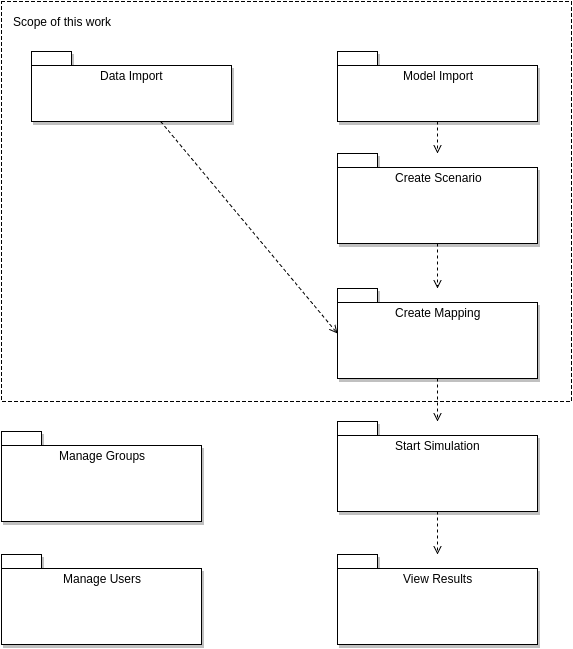
\includegraphics[width=.7\textwidth]{res/Dependency-workflow}
	\caption{Dependency workflow}
	\label{fig:dependency-workflow}
\end{figure}


\subsection{Data Import}
The data import lets the user add files to the system. These files feed the simulation with the information it needs. An example would be a time-series file that contains temperature values over time. The Websuite currently supports the following data types. All of the mentioned import types can be compressed inside a zip-file.

\subsubsection{Table-based}
This import type supports CSV-files with table data that refers to a specific GPS location. An Example would be the starting positions of agents in a model.

\subsubsection{Time-series}
The time-series import supports CSV-files with data that changes over time. An example is a layer, containing average temperatures per day over the duration of the desired simulation time.

\subsubsection{Geographic-Information-System (GIS)}
Data with a geographical representation can be imported with the GIS import. It supports the most common file types for GEO-processing, which are:
\begin{itemize}
	\item AciiGrid (*.asc)
	\item GeoTIFF (*.tif)
	\item GeoJSON (*.json)
	\item Shapefile (*.shp, *.shx, *.dbf and additional optional files)
\end{itemize}

\subsubsection{Grid-potential-field}
This data type allows the usage of potential-fields, which contains a grid of percentage values. These grids allow the calculation of distances to non moving objects prior to the simulation and hereby reduce simulation time. The file-ending is \textit{.csv}

\subsubsection{Geo-potential-field}
The Geo-potential-field layer is a specialized grid-potential-field layer that allows the use of GPS coordinates. The file-ending is \textit{.csv}.

\subsubsection{Obstacle-layer}
Obstacle-layer is a gird that contains obstacles. This can be used to limit agent movement. The file-ending is \textit{.csv}.


\subsection{Model Import}
The Model Import allows the upload of a zip-files, containing the DLLs of the model code. This is used in the scenario creation.


\subsection{Scenario Creation}
This step creates a scenario based on a previously uploaded model. During the creation, fields that need to be mapped, are determined in the following step .


\subsection{Mapping Creation}
Based on the scenario, the user maps fields for agents, layers and parameters to data imported by the data import or to manual values. This data is then validated with the back-end. Once the user has mapped all required fields successfully, it is possible to start the simulation. As shown in figure \ref{fig:dependency-workflow} that part will not be covered in this work.



\section{Interface Description}
The following section describes the REST calls, which are made by the WebUI to the different back-end services. The calls are separated by the components that call them.


\subsection{Dashboard (Home)}
The dashboard shows the user, what steps towards a successful simulation he has already completed.
\begin{table}[H]
	\caption{Endpoints used by Dashboard (Home)}
	\begin{tabularx}{\textwidth}{|l|X|}
		\hline
		\textbf{Endpoint} & \textbf{Usage} \\ \hline
		GET /metadata/metadata & Check if data \& model have been successfully imported. \\ \hline
		GET /scenario-management/scenarios & Check if a scenario has been created.\\ \hline
		GET /scenario-management/scenarios/\{id\}/complete & Check if a valid mapping exists.\\ \hline
	\end{tabularx}
\end{table}


\subsection{Data Import}
\begin{table}[H]
	\caption{Endpoints used by data import}
	\begin{tabularx}{\textwidth}{|l|X|}
		\hline
		\textbf{Endpoint} & \textbf{Usage} \\ \hline
		POST /file/files & Initiate data import.\\ \hline
		GET /metadata/metadata/\{dataId\}/state & Start long-polling. \\ \hline
	\end{tabularx}
\end{table}


\subsection{Model Import}
\begin{table}[H]
	\caption{Endpoints used by model import}
	\begin{tabularx}{\textwidth}{|l|X|}
		\hline
		\textbf{Endpoint} & \textbf{Usage} \\ \hline
		POST /file/files/models & Initiate model import. \\ \hline
		GET /metadata/metadata/\{dataId\}/state & Start long-polling. \\ \hline
	\end{tabularx}
\end{table}


\subsection{Scenario Creation}
\begin{table}[H]
	\caption{Endpoints used by scenario creation}
	\begin{tabularx}{\textwidth}{|l|X|}
		\hline
		\textbf{Endpoint} & \textbf{Usage} \\ \hline
		GET /scenario-management/scenarios & List all scenarios. \\ \hline
		GET /metadata/metadata & Show uploaded models during scenario creation and display  the model name in scenario list. \\ \hline
		POST /scenario-management/scenarios & Create a new scenario. \\ \hline
	\end{tabularx}
\end{table}


\subsection{Mapping Creation}
\begin{table}[H]
	\caption{Endpoints used by mapping creation}
	\begin{tabularx}{\textwidth}{|l|X|}
		\hline
		\textbf{Endpoint} & \textbf{Usage} \\ \hline
		GET /scenario-management/scenarios/\{id\} & Get the mapping structure. \\ \hline
		GET /metadata/metadata & Get data to map against. \\ \hline
		PUT /scenario-management/scenarios/\{id\}/mapping & Save the mapping. \\ \hline
		PUT /scenario-management/scenarios/\{id\}/parameter & save the parameters. \\ \hline
		GET /scenario-management/scenarios/\{id\}/complete & Check if mapping is complete and valid. \\ \hline
	\end{tabularx}
\end{table}


\subsection{Global}
\begin{table}[H]
	\caption{Endpoints used by global}
	\begin{tabularx}{\textwidth}{|l|X|}
		\hline
		\textbf{Endpoint} & \textbf{Usage} \\ \hline
		GET /metadata/metadata/\{dataId\} & Display the import processing as long-polling. \\ \hline
	\end{tabularx}
\end{table}
